\chapter{Context}
%Geef hier inzicht in het bedrijf/de organisatie waarvoor de opdracht wordt uitgevoerd. Denk in elk geval aan: beschrijving bedrijf/organisatie in je eigen woorden (geen teksten letterlijk overnemen van website), organogram of organisatiestructuur en indien relevant: organisatiestructuur van onderdeel waar opdracht betrekking op heeft.
Het afstudeerproject wordt uitgevoerd bij HeadForward (HeadForward B.V.) voor een van hun klanten, Allianz. HeadForward is een consultancy bedrijf en ontwikkelt, beheert en host maatwerk software en data- en integratie oplossingen. Met groep software professionals van hoge kwaliteit laat HeadForward opdrachtgevers in branches als de financiële dienstverlening, de overheid, de zorg, verzekeringen, industrie en landbouw, food \& retail vooroplopen in hun markt. 

Een van de klanten van HeadForward is Allianz Group en in dit project de externe opdrachtgever. De Allianz Group is een van oorsprong Duitse verzekeringsmaatschappij, met ruim 85 miljoen klanten in meer dan 70 landen en meer dan 147.000 medewerkers. 

Hierdoor heeft dit afstudeerproject een vlakke organisatiestructuur die tevens terug te zien is in het organogram (Figuur 3.1). De afdelingen waarin ik ga werken is Research en Development die direct wordt aangestuurd door ook de eindverantwoordelijke bij HeadForward, Dani\"el Siahaya. Dani\"el Siahaya communiceert vervolgens direct met Allianz.

\begin{figure}[ht]
    \begin{center}
        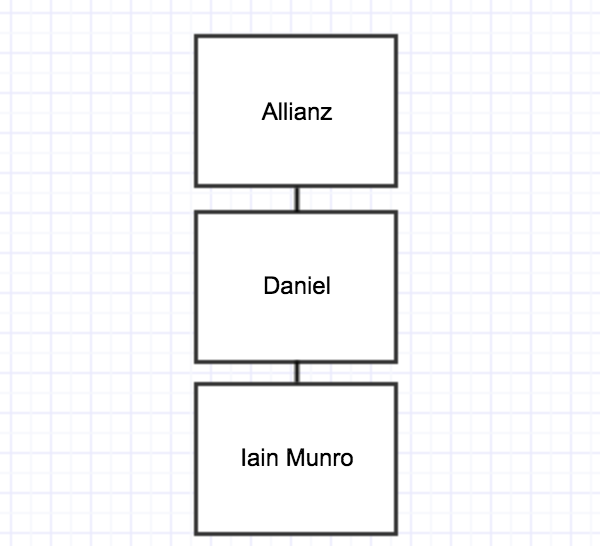
\includegraphics[width=200px]{images/org.png}
        \caption{organogram.}
    \end{center}
\end{figure}